\documentclass[12pt,a4paper]{article}
\usepackage[utf8]{inputenc}
\usepackage[russian]{babel}
\usepackage{amsmath}
\usepackage{amsfonts}
\usepackage{amssymb}
\usepackage{graphicx}
\usepackage{grffile}
\usepackage{subcaption}
\usepackage{float}
\usepackage[left=2.00cm, right=2.00cm, top=2.00cm, bottom=2.00cm]{geometry}
\begin{document}

	
	\begin{titlepage}
		\begin{center}
			\large
			ПРАВИТЕЛЬСТВО РОССИЙСКОЙ ФЕДЕРАЦИИ
			
			ФЕДЕРАЛЬНОЕ ГОСУДАРСТВЕННОЕ АВТОНОМНОЕ ОБРАЗОВАТЕЛЬНОЕ 
			
			УЧРЕЖДЕНИЕ ВЫСШЕГО ОБРАЗОВАНИЯ
			
			НАЦИОНАЛЬНЫЙ ИССЛЕДОВАТЕЛЬСКИЙ УНИВЕРСИТЕТ
			
			«ВЫСШАЯ ШКОЛА ЭКОНОМИКИ»\\[12pt]
			\vspace{0.25cm}
			
			МОСКОВСКИЙ ИНСТИТУТ ЭЛЕКТРОНИКИ И МАТЕМАТИКИ
			ДЕПАРТАМЕНТ ПРИКЛАДНОЙ МАТЕМАТИКИ
			
			\vspace{2cm}
			
			{\large Отчет 
				
				о прохождении преддипломной практики}
			\bigskip
		\end{center}
		\vfill
		
		\hfill\begin{minipage}{0.35\textwidth}
			Выполнил студент 4 курса\\
			С.\,В.~Колотев\\
			
			
			Научный руководитель\\
			Л.\,Н.~Щур\\
		\end{minipage}%
		\bigskip
		\vfill
		
		
		\begin{center}
			Москва, 2016 г.
		\end{center}
	\end{titlepage}
	
	\renewcommand\contentsname{Оглавление}
	\section{Введение}
	
	\par Исследование математических и физических свойств структурных образований на плоскости, а также распознавание появления фазовых переходов вызывает большой интерес на сегодняшний день. Это объясняется двумя факторами. Первый из них - научный. Развитие стохастической эволюции Левнера(позже названной как эволюцией Шрамма-Левнера), которая связывает свойства случайного блуждания в верхней полуплоскости со свойствами конформной теории поля(КТП). Она стала третьим подходом к алгебраическому решению (!!!) и КТП (!!!) решения для нахождения критических свойств некоторых двумерных системы классической статистической физики. Успешными примерами данного подхода являются задача о перколяции и модель Изинга. Второй фактор - это исследование физических и математических процессов планарной геометрии, связанных с практикой разработки новых материалов для микроэлектронных устройств следующего поколения. Для объяснения конформной теории поля, сначала необходимо пояснить, что такое квантовая теория поля. 
	
	\par Квантовая теория поля изучает характеристики элементарных частиц, а также процессы взаимодействия между ними, а свойства самих частиц описываются с помощью теории относительности. Несмотря на различные происходящие процессы между элементарными частицами, их физические характеристики остаются неизменными. Если ввести конформные(т.е. сохраняющие углы в точках пересечениях кривых) преобразования, то конформная теория поля - это инвариантная относительно конформных преобразований квантовая теория поля. Благодаря инвариантности, в КТП можно решить задачи, которые довольно сложно или невозможно решить в квантовой теории поля.
	
	\par Эволюция Шрамма-Левнера(SLE)  была впервые представлена в 1999г О. Шраммом. Это однопараметрическое семейство мер на прямых без самопересечений. Было показано, что на некоторых дискретных случайных блужданиях на решетке (например,случайное блуждание по петле[16], критический перколяционный проводник [28, 6]) имеют SLE как предел масштабирования. 
	\par Конформные преобразования можно использовать для описания кривой без самопересечений, растущей с границы односвязной области. Отображение переводит область с кривой в область без кривой внутри.
	\begin{equation}\label{assymp}
		g_{t}(z) ~ z + 2t/z + O(1/z^{2})
	\end{equation}
	
	\par Формулой \ref{assymp} описывается асимптотика отображения. Где $t$ - является параметром. Если кривая касается саму себя, то отображение должно переводить в область, но уже без объединения кривой и тех точек, которые невозможно достичь из бесконечности. Левнер установил, что с помощью положения образа крайней точки можно определить как функцию $g_{t}(z)$, так и саму кривую, для этого нужно решить дифференциальное уравнение Левнера 
	\begin{equation}\label{sle_eq}
		\dfrac{dg_{t}(z)}{dt} = 2[g_{t}(z)-\xi(t)]^{-1}
	\end{equation}
	\par О. Шрамм показал, что мера инвариантна на кривых лишь при выполнении равенства \ref{invar}
	
	\begin{equation}\label{invar}
		\xi(t) = \sqrt{k}B_{t}
	\end{equation}
	 - где $\xi(t)$ - образ кривой точки или управляющая функци, $k$ - параметр кривизны кривой, $B_{t}$ - одномерное броуновское движение.
	\par Существуют два вида эволюции: хордальная и радиальная. Чаще всего исследования проводятся на первом типе, который описывает кривые, соединяющие один простой конец с другим в односвязной области. Второй тип представляет собой двустороннюю радиальную функцию и функцию Грина. Двусторонняя радиальная функция делится на две части. Первая - от простого конца во внутреннюю точку, а вторая - из внутренней точки ко второму просто концу. Иными словами, это кривая представляет собой хорду через фиксированную внутреннюю точку. Функция Грина оказалась плотностью SLE кривой с естественной параметризацией. Таким образом двусторонняя радиальная кривая соответствует дискретному случайному пути, а функция Грина - плотности пути. 
	
	
	\par Что же такое задача о перколяции? В статистической физике существует раздел, называемый "Теория перколяции", которая занимается изучением поведения связных структур на случайных графах. Основным вопросом, которым занимается эта теория заключается в следующем: можно ли пройти от одного конца графа к другому по его элементам. Соответственно разделяют на перколяцию по узлам и перколяцию по связям. В наши дни теория перколяции имеет довольно широкое применение. В качестве примера можно привести ситуации из жизни. Как близко нужно садить деревья в лесу, чтобы, в случае пожара, огонь не сможет перекинуться на близлежащие деревья? Или же когда поливают пористый материал какой-нибудь жидкостью, достигнет ли она дна? В сфере медиа например, определить доступность той или иной машины в сетевом сегменте.
	
	\par Перейдем к модели Изинга. Пусть на двумерной решетке находятся точки, которые имеют определенной состояние, называемое "спин". Он может быть повернут вверх или вниз. Значению "вверх" соответствует +1, а "вниз" -1. Задав каждой точке свое спиновое число, получается конфигурация решетки. У конфигурации есть характеристика, называемая "энергией конфигурации" - она равна сумме произведений всех соседних пар точек,
	\begin{equation}\label{conf_energy}
		E({\sigma}) = - \sum_{(ij)}J_{ij}^{x}\sigma_{i}\sigma_{j} -\sum_{(ik)}J_{ik}^{y}\sigma_{i}\sigma_{k}
	\end{equation}
	
	- где $\sigma$ - конфигурация решетки, $\sigma_{i}$ - точка на решетке, имеющая спин, ($ij$) - сумма по строке и ($ik$) - сумма по столбцу, $J$ - константа связи, являющейся параметром взаимодействия между точками. Статистическая сумма - одна из важных и полезных характеристика в статистической физике. Статсумма представляет собой функцию от температуры, позволяющую получить сведения об энергии, энтропии и других свойствах системы в термодинамическом равновесии. 
	\begin{equation}\label{statsum}
		Z = \sum_{\{\sigma\}}e^{E(\{\sigma\})/T}
	\end{equation}
	- где $T$ - температура, $E(\{\sigma\})$ - энергия конфигурации
	
	\par В теории фазовых переходов наиболее исследуемыми на текущий момент являются переходы первого и второго рода. Для фазового перехода первого рода характерно изменение границы $I$ между двумя структурами разного типа как линейная функция $I \sim L$, зависящая от размера системы. Для фазового перехода второго рода граница изменяется как степенная функция размера системы $I \sim L^{\theta}$. Пару лет назад начали рассуждать на тему смешанного фазового перехода, в котором одни наблюдаемые величины ведут себя как при фазовом переходе первого рода, а другие - как второго. Аналитические исследования смешанного фазового перехода были проведены на одномерной системе. В обычной задаче о перколяции вероятность принадлежать к бесконечной структуре(кластеру)	подчиняется степенной функции от параметра модели. Затем было высказано предположение о том, что в динамической перколяции эта вероятность может резко меняться как функция параметра, известного как "discontinuous percolation" или разрывная перколяция. 
	
	\section{Постановка задачи}
	
	\par Основной целью данной работы является найти ответ на вопрос - как меняются геометрические свойства стационарных или квазистационарных случайных структур?
	
	\par Для этого необходимо смоделировать пространственную эволюционную игру "Дилемма узника" на квадратной решетке с периодическими граничными условиями. В которой каждый агент принимает одну из двух стратегий - кооператор (C) или дефектор (D). Начальная конфигурация случайна. Но для начала необходимо ознакомиться с самой моделью, какие вариации бывают и для чего они используются.
	
	\section{Модели теории игр}
	
	\par Середина XX века примечательна многими событиями, одним из которых является
	развитие теории игр. Основная цель классической теории игр заключается в поиске
	оптимальной стратегии в игре между двумя и более игроками, каждый из которых может
	определять свое поведение. В повторяющейся игре агенты играют несколько раз по 
	тем же правилам. Благодаря этому можно проследить изменения в поведении игрока,
	которое наблюдается из-за того, что он принимает то или иное решение исходя из
	результата предыдущих игр. Иными словами, его стратегия эволюционирует. 
	
	\par Существует множество моделей теории игр, которые являются объектом исследования ученых и по сей день.
	
	\par "Ультиматум" - одна из самых простых моделей теории игр, придумана в 1982г. Между двумя агентами необходимо поделить сумму денег. Один из них предлагает кому сколько достанется, второй же игрок либо соглашается с вариантом и получает свою часть, либо отвергает предложение и деньги никому не достаются. 
	
	\par Модель "Трагедия общинного поля" была придумана ещё в первой половине XIXв Уильямом Фостером Ллойдом. Есть поле, на котором деревенские жители пасут коров.
	Если у всех будет пастись по одной корове, то в этому случае всё будет хорошо, травы на поле хватит, если у кого-то появится вторая корова, то это тоже не критично. Но если каждый житель обзаведется по еще одной корове, тогда на поле не останется травы и весь скот умрет от голода. 
	\par "Проблема вагонетки" состоит в том, готов ли человек толкнуть на рельсы человека, ради спасения вагонетки с пассажирами. Предложена в 1967г Филиппой Фут. 
	
	\par "Аукцион". На продажу выставляется купюра и как и в обычном аукционе происходят торги, в которых участники называют свою цену. Купюру забирает тот, чья ставка была максимальной, но есть один ньюанс - владелец купюры помимо суммы ставки получает также ставку предшествующей максимальной. 
	
	\par Одна из самых распространенных моделей теории игр является Дилемма Заключенного.
	В ней играют два агента, каждый из которых использует две возможные стратегии: 
	кооператор C и дефектор D. Агент получает определенное количество очков от выбора
	своей стратегии и стратегии своего оппонента.
	
	\subsection{Виды модели Дилеммы узника}
	\par У повторяющейся Дилеммы Заключенного также существуют вариации, влияющие на то, как будет эволюционировать поведение агентов, какую стратегию они выберут в той или иной ситуации. Кроме того, модель может иметь большее число стратегий, чем в стандартной интерпретации. Ниже приведены некоторые из них.
	
	\par В одной из вариаций каждый агент со стратегией кооператора всегда будет кооператором на протяжении всей игры и только дефекторы имеют возможность выбора стратегии. Или же ситуация наоборот - когда только кооператоры могут поменять стратегию, а дефекторы остаются дефекторами на протяжении всего времени. 
	
	\par Существует вероятностная модель, в которой вводится некий случайный параметр, отвечающий за то, какую стратегию выберет агент в следующей игре.
	
	\par Также есть модель, в которой агент копирует поведение своего оппонента. Она имеет название "око-за-око". Помимо этого, агент может взять стратегию оппонента, если он дважды выбрал одну и ту же, или наоборот - придерживаться предыдущей стратегии оппонента несколько игр подряд.
	
	\par Существуют и более хитрые вариации. Например, если одна из стратегий принесла агенту хороший доход(после игры с кооператором, если он был кооператором или дефектором), то он будет ее придерживаться, пока она не принесет ему плохой доход. После чего он сменит стратегию и также будет ориентироваться на доход от новой стратегии. 
	
	\par Более того, есть модель, в которой агент придерживается стратегии кооператора, если его оппонент за все предыдущие игры был чаще кооператором, чем дефектором. Здесь приходится определять, что делать, когда оппонент принимал обе стратегии одинаковое количество раз. 
	
	\par Интересно задуманы следующие две модели. В первой агент рассчитывает долю игр оппонента как дефектора и использует ее в качестве вероятности принять данную стратегию самому. Во второй модели агент, прежде чем начинать рассчитывать вышеописанную долю, играет за кооператора некоторое количество игр, затем копирует поведение оппонента, и лишь только потом приступает к вычислению вероятности.
	
	\par Эволюционная теория игр исследует поведение большой популяции, где макроскопическое
	число игроков имеет конечное число стратегий. В то время как классическая теория игр имеет дело с одиночными агентами. Пространственная эволюционная игра заключается в помещении агентов на какую-либо пространственную структуру и во взаимодействии их со своими ближайшими соседями. Структуры могут быть разнообразными - решетки, графы, сети. В качестве модели в текущем исследовании была взята пространственная эволюционная Дилемма Узника на двумерной решетке.
	
	\par Пространственное расположение игроков образует геометрические структуры - группы игроков, которые синхронизируют свое поведение с соседями и конкурируют с другими группами.
	 
	\section{Исследование детерминистической модели}
	
	\subsection{Алгоритм Хошена-Копельмана}
	
	\par Для решения задачи о перколяции был ученые Дж. Хошен и Р. Копельман придумали алгоритм, который позволяет выделить различные структурные образования на решетке или графе. Одним из замечательных свойств данного алгоритма является то, что он позволяет разбить решетку на кластеры можно всего за один проход по ней. В условиях большого размера системы это несомненно является большим преимуществом. На выходе после работы алгоритма можно узнать к какому кластеру принадлежит тот или иной агент на решетке, а также размер каждого кластера.
	
	\par Принцип алгоритма довольной простой. В качестве примера будем рассматривать изучаемую модель, т.е. квадратную решетку с периодическими граничными условиями. Сразу стоит сказать, что в изначальной версии алгоритма учитываются только соседи по горизонтали или вертикали, как ладья, но лишь на соседнюю клетку. А так как в модели каждый агент взаимодействует с агентами и по диагонали, то необходимо при работе алгоритма рассматривать и их. Таким образом, при разбиении на кластеры каждый агент аналогично королю из шахмат смотрит на соседей. На Рис.\ref{hkpic} представлена иллюстрация работы алгоритма Хошена-Копельмана без каких-либо модификаций.   
	\par В нашем случаем мы начинаем проход по строкам, начиная с левого верхнего агента. Можно начать с каждого конца и идти, например, по стоблцам - суть алгоритма от этого не изменяется. Цель - правильно расставить метки на агентах. Эти метки соответствуют кластеру, к которому принадлежат данные агенты. Каждой метке соответствует индекс элемента массива кластеров, а сами элементы кластера - это его размер, или иными словами - количество агентов, помеченных номером соответствующего кластера.
	\par В самом начале, когда решетка не заполнена, на первой строке агент смотрит на предыдущего, принадлежит ли тот какому-либо кластеру, если да, то текущий агент маркируется также, как и его сосед. Если предыдущий не имеет метку или является другим типом элемента, то номер метки увеличивается на единицу. Первая строка разбивается быстро и просто. 
	\par Что касается второй строки и последующих, то там есть некоторое дополнение. Каждый агент должен смотреть на соседа слева, и на троих соседей сверху. И вот здесь происходит наиболее сложная логика алгоритма, так как вероятно, что среди этих агентов найдутся те, которые принадлежат разным кластерам. В этом случае предпочтение отдается текущий агент присоединится к кластеру с наименьшей меткой среди соседей. Кроме того, два конкурирующих кластера должны объединиться в один, так как текущий агент является их общим элементом. 
	\par Объединение двух кластеров происходит лишь на уровне массива с размерами. Кластер с большей меткой присоединяется к тому, что с меньшей, их размеры суммируются, а в массиве на место элемента кластера с большей меткой помещается номер метки кластера, в которой произошло слияние, причем со знаком минус. Таким образом в массиве создается связь между двумя кластерами, и если мы хотим узнать, какому кластеру принадлежит элемент, то можно посмотреть на его метку, и если в массиве под таким индексом лежит отрицательное число, то оно указывает на метку кластера, к которому было присоединение.
	
	\par Необходимо учитывать ситуацию, происходящую на границе решетки. Так как в текущей модели периодические границы, то необходимо, чтобы каждый крайний агент проверял другую сторону решетки на наличие метки.
	\begin{figure}[H]
		\centering
		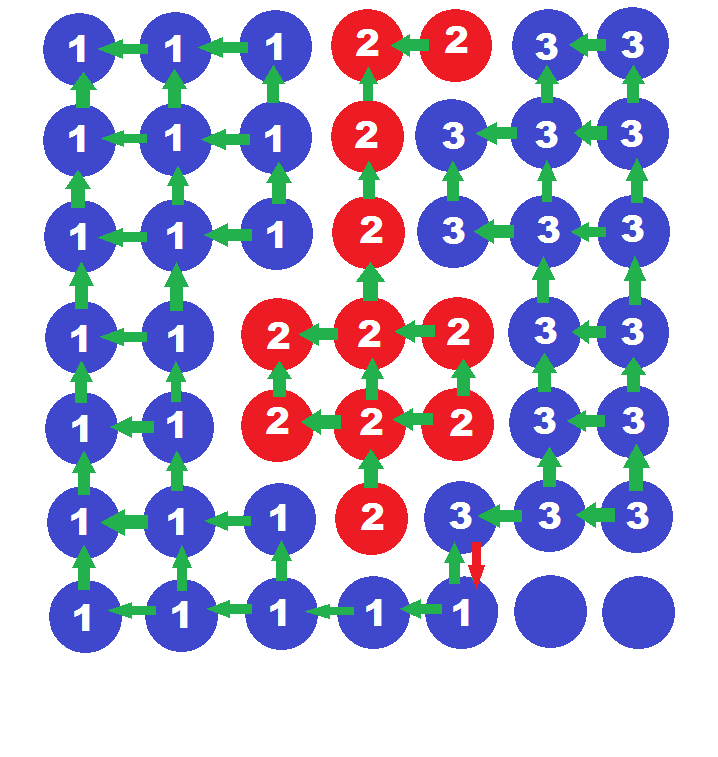
\includegraphics[width=0.5\linewidth]{HKpic2.png}
		\label{hkpic}
		\caption{Принцип алогритма HK76. Зеленые стрелки показывают, на каких соседей смотрит текущий агент. Красная стрелка показывает ситуацию слияния одного кластера в другой}
	\end{figure}
	
	
	\subsection{Описание модели}
	\par В этой работе исследование модели Дилеммы Узника началось с варианта Р.Мэя и М.Новака. Ученые расположили агентов на квадратно двумерной решетке. Для минимизации граничных эффектов были взяты периодические граничные условия. Начальная конфигурация составляет $90\%$ кооператоров. Каждый агент играет с восемью ближайшими соседями и с самим собой, получая при этом определенный доход. В следующем раунде агент возьмет стратегию с максимальным доходом среди соседей или же свою(если его стратегия была более прибыльная).
	
	\par В элементарной игре количество очков зависит от выбранной стратегии. Ученые определили следующие правила:
	\begin{itemize}
		\item если оба агента дефекторы, то никто ничего не получает
		\item если оба кооператоры, то оба получают доход $S=1$
		\item при игре разных стратегий дефектор получает максимальный доход $T>S$, а кооператор ничего
	\end{itemize}
	
	
	
	
	\par Ученые пришли к выводу, что данная модель является клеточным автоматом, в котором состояние агентов зависит от окружающих его соседей, которые также зависят от своего окружения. Таким образом, в определении состояния агента в следующем раунде влияет 25 окружающих его агентов. На Рис. \ref{parall} в черной рамке показаны соседи, между которыми агент будет выбирать стратегию, а те, что в зеленой рамке участвуют только в подсчете дохода. Получается 2 уровня соседей и его текущее состояние. Также примечателен тот факт, что доход зависит только от одного параметра $b=T/S$. 
	
	\par Кроме того, было изучено поведение единичного агента среди агентов другой стратегии. Так при $b<1$ дефекторы исчезают всегда, а $b>3$ вымирают уже кооператоры. При $1<b<9/5$ возникают описанные учеными некоторые структурные образования, названные глайдерами, ротейторами и гроверы. Малые структурные образования остаются не увеличиваются, а большие становятся меньше. Но в ситуации, когда $b>9/5$ единичный дефектор и любая структура из дефекторов начинает расти, причем единичный дефектор начинает расти как калейдоскоп, что выглядит довольно красиво. Что касается кооператоров, то они растут до того момента, когда $b<2$, и большие структурные образования из кооператоров уменьшаются при $b>2$. Можно заметить, что среди промежутков роста и тех и других агентов, есть промежуток, в котором растут структуры как кооператоров, так и дефекторов, поэтому там и наблюдается некое соперничество между обеими стратегиями.
	
	\subsection{Границы интерфейса}
	
	\par Целью работы - выяснить, как изменяются геометрические свойства структур на решетках. Для этого необходимо ввести понятие интерфейса или границы кластера. Само слово интерфейс, известное многим, означает средство или инструмент взаимодействия одного объекта с другим. Например, человек взаимодействует с компьютером, управляя мышью или клавиатурой. Но в данной ситуации это не средство управления, а скорее то, что находится между двух различных сред, поэтому сюда больше подходит понятие границы.
	
	\par Для определения понятия границы, нужно объяснить, что такое дуальная решетка. Возьмем обычную квадратную решетку, аналогичную той, что в модели этого исследования и наложим на неё еще одну такого же типа, но таким образом, чтобы ее ребра проходили через середины ребер первоначальной решетки и были им перпендикулярны. Такая конструкция называется и дуальной решеткой.
	
	\par Так как мы наша задача тесно связана с задачей о перколяции, то исследовать геометрические свойства необходимо у протекающих кластеров. Это те кластеры, по элементам которого можно дойти от одной границы решетки к противоположной. Данные кластеры из-за периодических граничных условий являются бесконечными, поэтому они и интересны. 
	
	\par Теперь перейдем непосредственно к объяснению, что же такое граница. Проведем связи между крайними элементами протекающего кластера к соседям, имеющих другую стратегию. Элемент называется крайним, если по горизонтали или по вертикали среди его соседей найдется хотя бы один агент, имеющий другую стратегию. Теперь вернемся к дуальной решетке и проведем перпендикулярно этим связям линию, соединяющую узлы дуальной решетки. Совокупность этих линий является границей или интерфейсом протекающего кластера. На Рис.\ref{bord} изображен пример как выглядит граница протекающего кластера из дефекторов.
	
	\begin{figure}
		\label{bord}
		\centering
		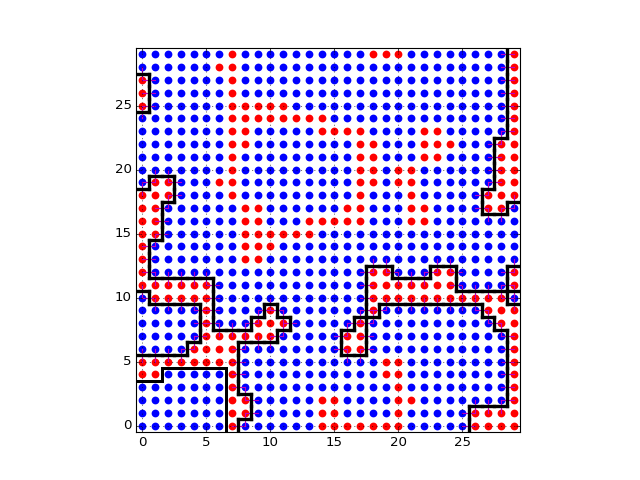
\includegraphics[width=0.7\linewidth]{border2.png}
		\caption{Пример границы протекающего кластера из дефекторов}
	\end{figure}

	\par Численная величина границы - это количество линий, проведенных перпендикулярно связям между элементами протекающего кластера и агентами другого типа. Количество линий - это фактически число связей, через которые они были проведены, а это равно количеству соседей, имеющих другую стратегию. Таким образом алгоритм вычисления границы заключается в следующем. Идем построчно начиная с верхнего левого элемента решетки. Проверяем, принадлежит ли он протекающему кластеру. Если да, то считаем количество его соседей по вертикали и горизонтали, которые имеют другую стратегию, затем переходим к другому элементу. 
	
	\subsection{Ускорение расчетов}
	
	\par В этом разделе будет описан алгоритм ускорения смены конфигурации в модели. Очевидно, что увеличение размера системы требует серьезных затрат с точки зрения производительности, поэтому для вычисления на системах с разными размерами мы разработали параллельный алгоритм подсчет конфигурации системы.
	
	\par Для ускорения работы алгоритма мы выбрали OpenMP. Довольно простой принцип использования, которые не требует серьёзной модификации основного алгоритма позволяет получить существенный прирост производительности.
	
	\par В технологии OpenMP существует главная нить, называемая "мастер", в которой выполнение кода происходит последовательно. Но эта нить порождает дочерние и разделяет между ними те части кода, которые необходимо распараллелить. 
	
	\par Для модернизации кода необходимо поместить нужны директивы в части когда. А для использования нужно лишь задать соответствующий ключ при компиляции программы. Это также большой плюс в гибкости кода - легко переключаться между параллельной и последовательной версией программы. Но для OpenMP необходимы системы с общей памятью, а также компилятор, поддерживающий соответствующую технологию.
	
	\par Одной из целей параллельного программирования является распределение однотипных инструкций процессору между нитями. Засчет этого и получается ускорение. Следуя этому принципу, мы распараллелили модель эволюционной игры. Мы распределили между нитями каждую строку решетки, как показано на Рис.\ref{parall} и получили соответствующий прирост в скорости выполнения программы. На Рис. показано время работы последовательного кода и варианта с использованием технологии OpenMP.
	
	\begin{figure}
		\label{time}
		\centering
		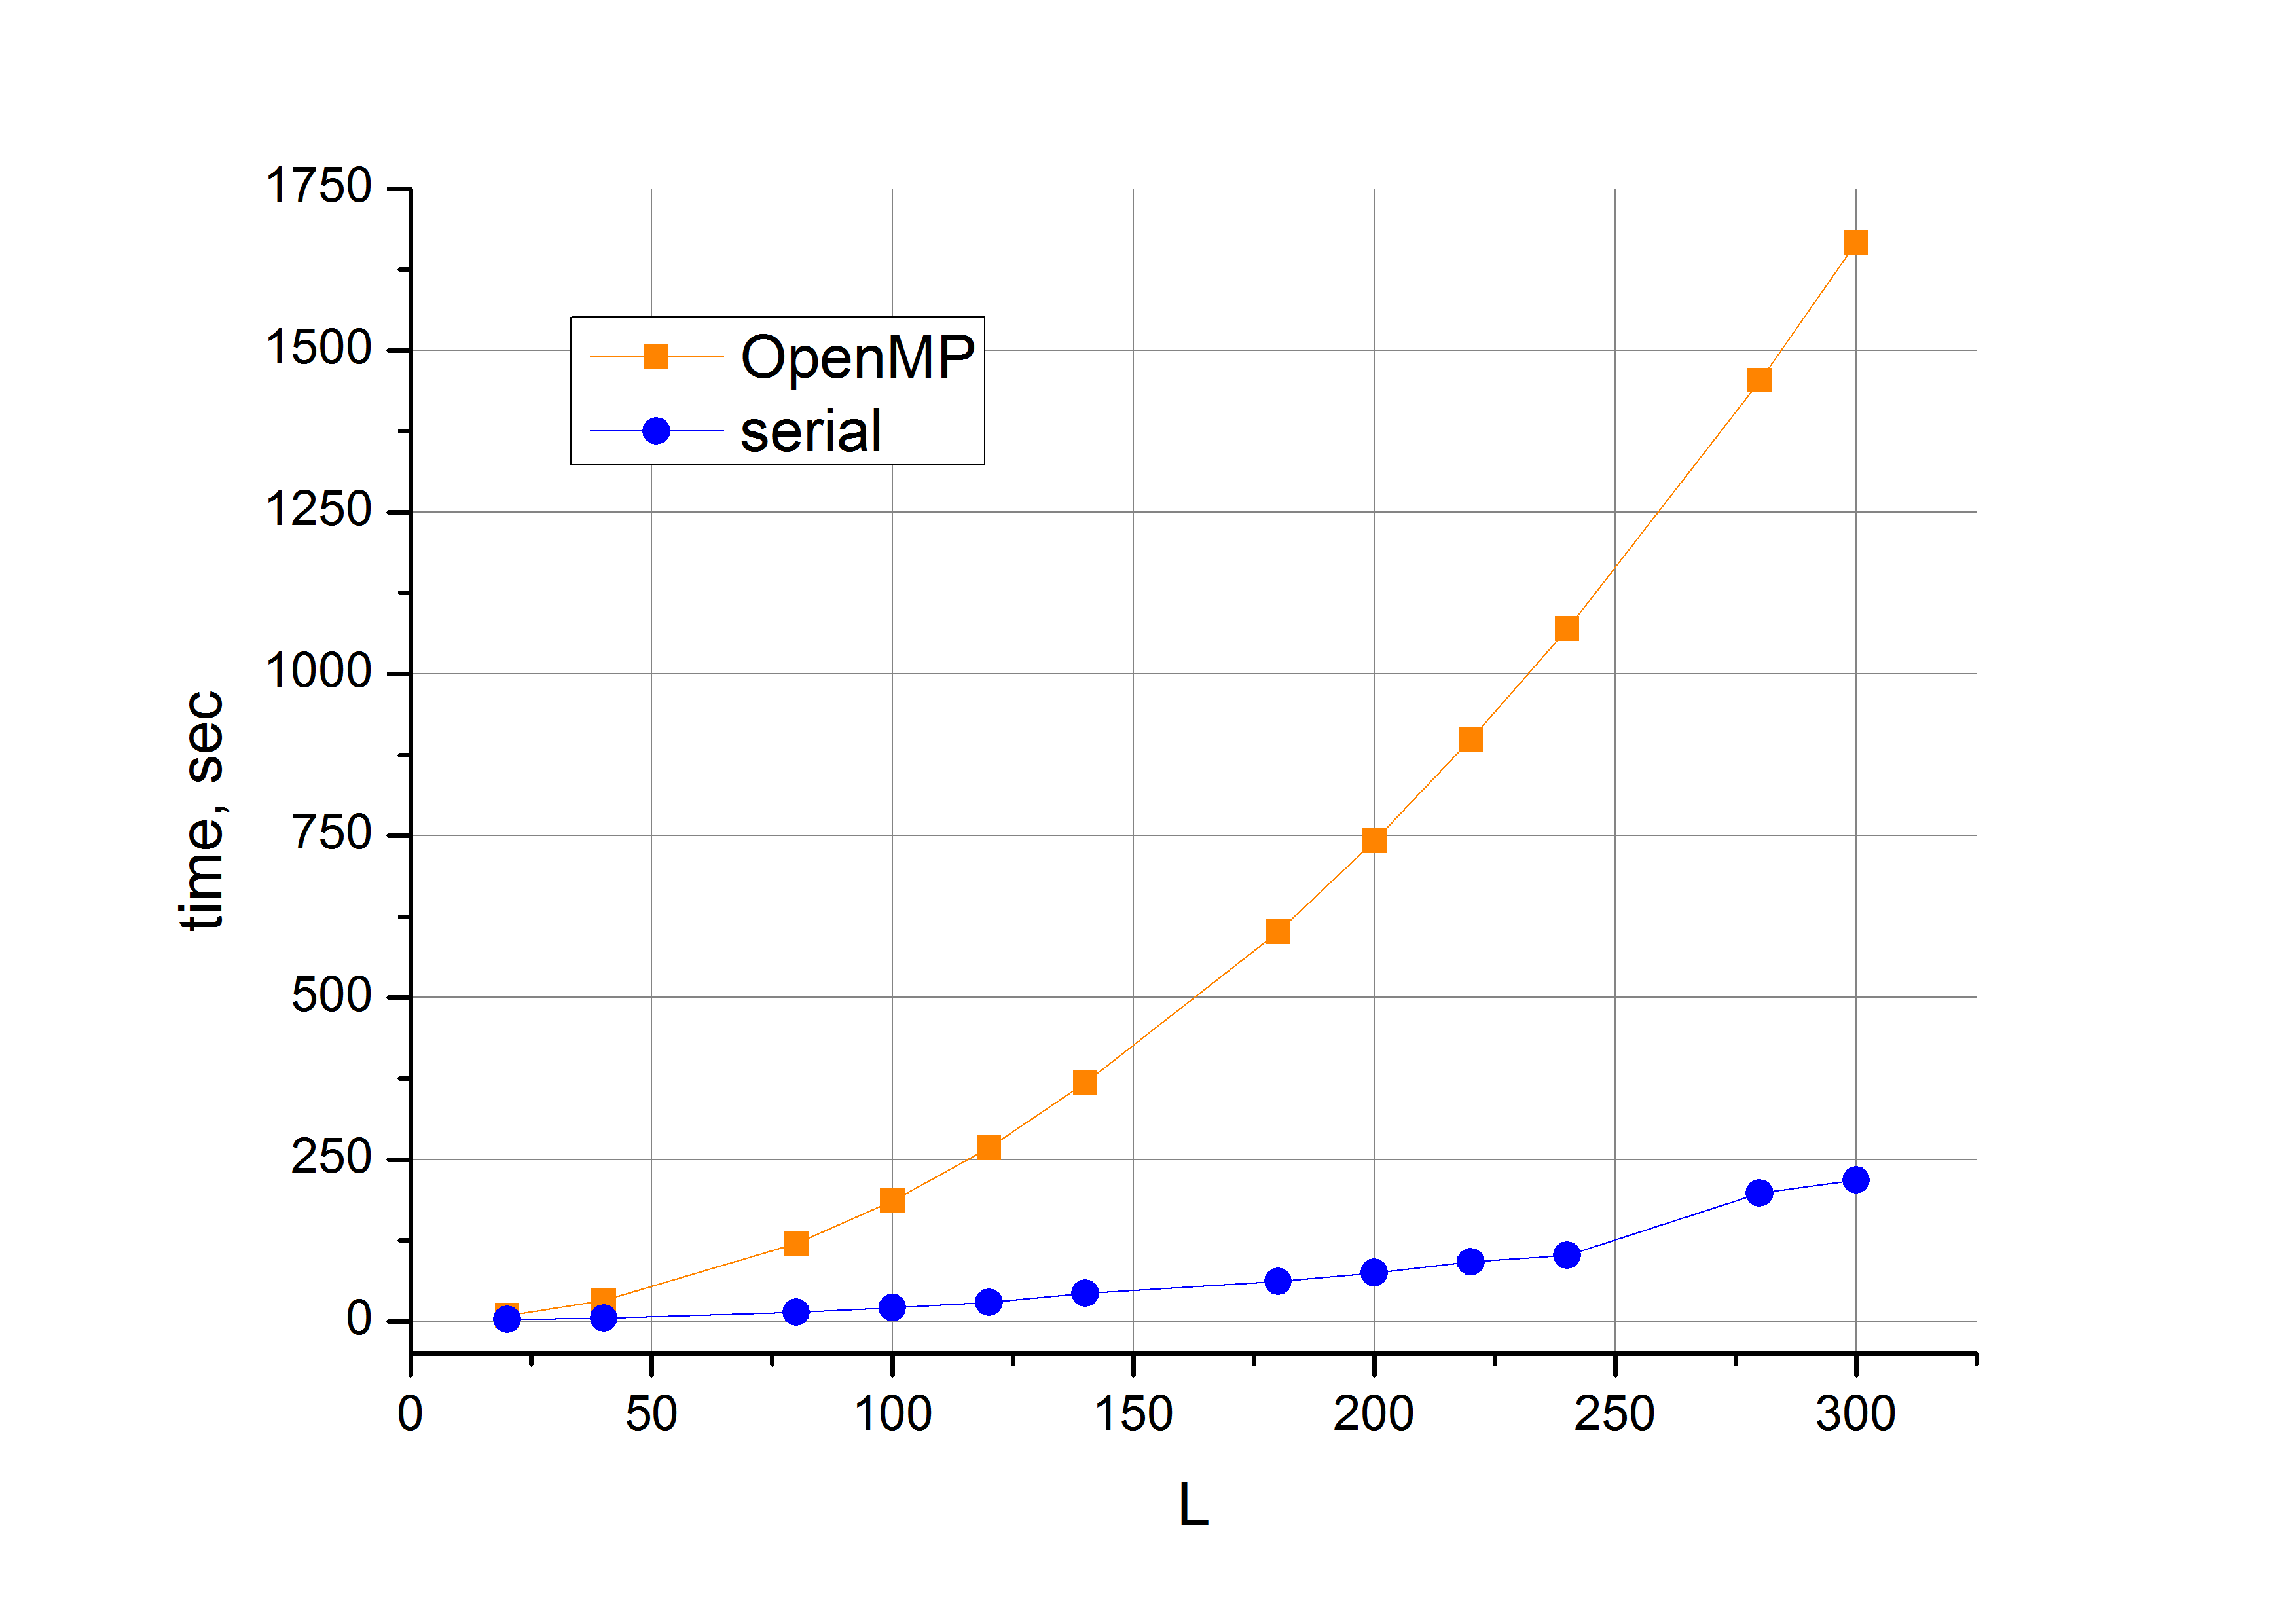
\includegraphics[width=0.7\linewidth]{time.png}
		\caption{Время выполнения последовательного и параллельного алгоритма в сек. По вертикали - время выполнения в сек. По горизонтали - размеры решетки.}
	\end{figure}
	
	\begin{figure}[H]
		\label{parall}
		\centering
		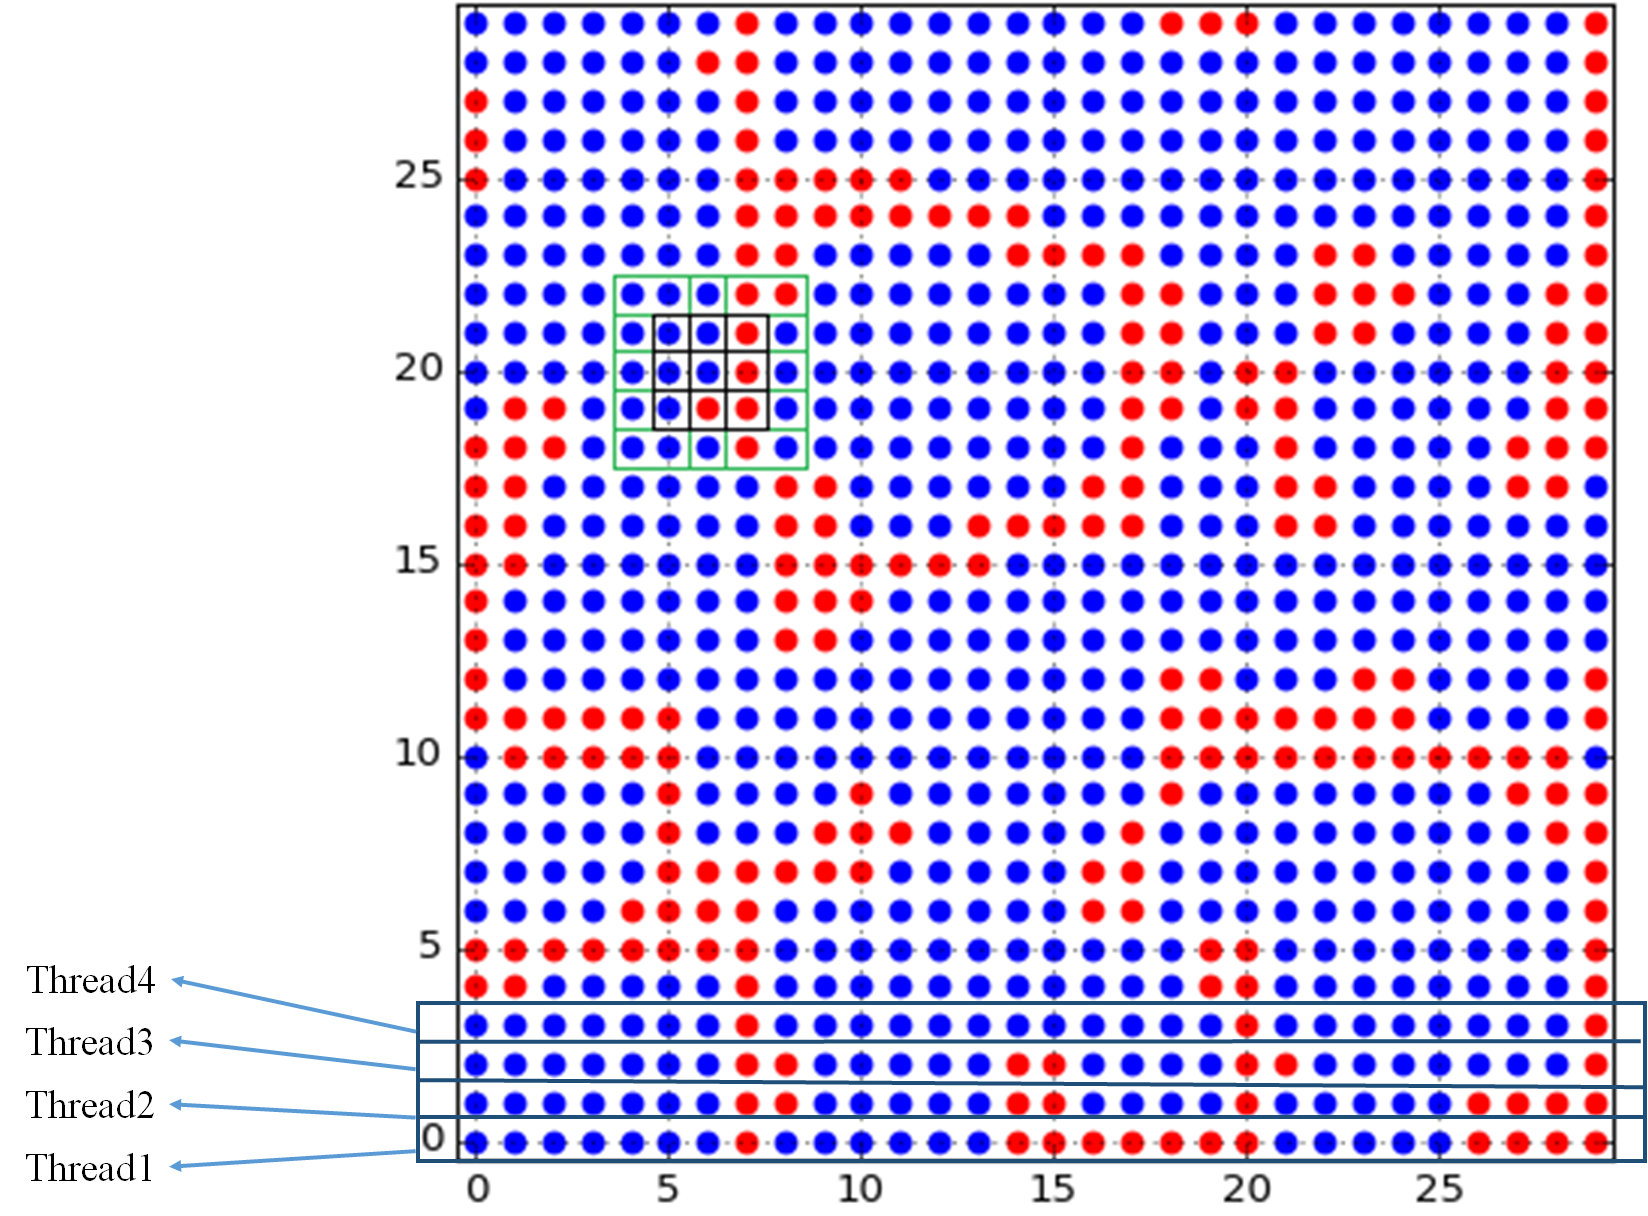
\includegraphics[width=0.7\linewidth]{rule.png}
		\caption{Иллюстрация параллельного алгоритма и количества игроков, участвующих в определении стратегии.}
	\end{figure}
	
	\section{Вычисления}
	
	\par Исследуя пространственную эволюционную Дилемму Узника Р. Мэя и М. Новака, удалось выявить, что конфигурация агентов на решетке резко меняется при переходе через значение $b = 9/5$. При $b<9/5$ структура кооператоров относительно статична, а при $b>9/5$ наоборот можно наблюдать разнообразную динамику на решетке - рост, передвижение и столкновение.
	
	\par Для наглядного представления, как меняется динамика игры с изменением параметра $b$, было взято 25 независимых реализаций начального заполнения и вычислена средняя плотность кооператоров по времени, без учета первых $10^{3}$ игр для уравновешивания и усреднения по $2 x 10^{4}$ раундов. На Рис. показан график изменения плотности кооператоров от параметра $b=T/S$, на котором отчетливо виден резкий переход в точке $b=9/5$, при котором плотность кооператоров падает с $~70\% $ до $~30\%$
	
	\begin{figure}[H]
		\label{freq}
		\centering
		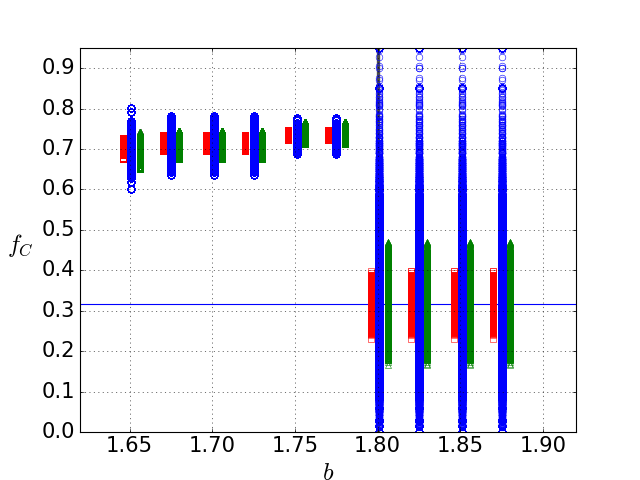
\includegraphics[width=0.7\linewidth]{fig1_1.png}
		\caption{Изменение плотности кооператоров от параметра $b$}
	\end{figure}
	
	\par Так же можно заметить одну особенность. Не только плотность изменяется при  переходе через особую точку, также распространение мелких структур резко увеличивается. Но несмотря на это, оно имеет конечный размер, уменьшающий с ростом размера всей решетки. Второй факт заключается в том, что средняя плотность кооператоров на решетке при $b>9/5$ удовлетворяет значению $ f_{C} = 12log2-8 \approx 0.32$.
	
	\subsection{Простая модель со случайным полем}
	
	\par Моделируется пространственная эволюционная игра на основе модели
	Дилеммы Узника, помещенная на квадратную решетку с периодическими граничными
	условиями, в узлах которой находятся игроки одного из двух типов - кооператор 
	или дефектор. Каждый игрок получает доход, играя со своими 8 соседями и со средним полем. Среднее поле определяется следующим образом - вычисляется доля кооператоров на решетке в данный момент времени, генерируется число в интервале от 0 до 1 и сравнивается с долей кооператоров. Если оно оказалось больше, то девятый игрок - дефектор, если меньше - кооператор. В следующем раунде игрок выберет стратегию соседа с максимальным доходом. Случайный игрок окажется кооператором с вероятностью
	равной плотности кооператоров на решетке в данный момент времени. Решетка 
	обновляется, когда каждый игрок определил свой тип в следующем раунде.
	
	\par Ниже в приведены формулы, по которым рассчитываются доходы кооператора ($P_{c}$) и дефектора ($P_{D}$)
	
	$ P_{c}= n_{c}*R+ \theta(f_{c}-x) $
	
	$ P_{D}= n_{c}*R*b+ \theta(f_{c}-x)*b $
	
	где $ f_{c}$ - плотность кооператоров на решетке в данный момент
	времени, $\theta(f_{c}-x)$ - функция Хэвисайда, $x \in [0,1]$- случайное число
	$n_{c}$ - количество соседей, являющихся кооператорами
	 
	
	\par Эта модель практически совпадает с той, что описали в своих работах Р. Мэй и
	М. Новак в 1992г. Отличие составляет лишь то, что в их версии игрок вместо случайного
	игрока играет сам с собой.
	
	\par На \ref{fig:1} представлен пример динамики, происходящей на решетке за 4 поколения.
	Размер решетки 50х50 игроков, параметр $b=1.51$ синим цветом обозначены кооператоры, красным - дефекторы. 
	\begin{figure}[H]
		\centering
		\begin{subfigure}{.5\textwidth}
			\includegraphics[width=1\linewidth]{../conf/grids/pics/2}
			\caption{}
		\end{subfigure}%
		\begin{subfigure}{.5\textwidth}
			\includegraphics[width=1\linewidth]{../conf/grids/pics/3}
			\caption{}
		\end{subfigure}%
	
		\begin{subfigure}{.5\textwidth}
			\includegraphics[width=1\linewidth]{../conf/grids/pics/4}
			\caption{}
		\end{subfigure}%
		\begin{subfigure}{.5\textwidth}
			\includegraphics[width=1\linewidth]{../conf/grids/pics/5}
			\caption{}
		\end{subfigure}%
		\caption{Снимки решеток игры со случайным игроком 50х50 при $b=1.51$}
		\label{fig:1}
	\end{figure}
	
	В приложении находятся графики зависимости плотности кооператоров на решетке 
	от времени при различных значениях параметра $b$. Зеленым цветом показано поведение
	модели Р.Мэй и М.Новака. Синим - модель со случайным игроком. Начальное заполнение решетки 90$\%$ игра длится 21000 поколений. Можно заметить, что сначала присутствует резкое падение вниз плотности кооператоров, а затем с определенного момента изменение 
	стабилизируется, причём для каждого параметра $b$ время релаксации является различным.
	
	\par При подсчете средних плотностей первоначальные изменения плотности не учитываются, поэтому начало подсчета начинается со значений, указанных в \ref{tab1}, где $t_{old}$ - время релаксации в модели Р.Мэй и М.Новак,  $t_{new}$ - в модели со случайным игроком,
	$b$ - максимальный доход в одной игре между двумя игроками.
	
	
	\vspace{10px}
	\begin{center}
	\begin{table}[H]
	\centering
		\begin{tabular}[H]{|c|c|c|}
			\hline 
			b&$t_{old}$& $t_{new} $ \\
			\hline 
			1.3& 100 & 10000 \\ 
			\hline 
			1.35& 100 & 16000 \\ 
			\hline 
			1.4& 100 & 2000 \\ 
			\hline 
			1.45& 100 & 500 \\ 
			\hline 
			1.5& 400 & 100 \\ 
			\hline 
			1.55& 400 & 500 \\ 
			\hline 
			1.6& 16000 & 100 \\ 
			\hline 
			1.65& 100 & 500 \\ 
			\hline 
			1.7& 100 & 4000 \\ 
			\hline 
			1.75& 100 & 1000 \\ 
			\hline 
			1.8& 100 & 500 \\ 
			\hline 
			1.85& 100 & 500 \\ 
			\hline 
			1.9& 100 & 500 \\ 
			\hline 
		\end{tabular}
		\label{tab1}
		\caption{Время релаксации при различных параметра $b$}
	\end{table}
	\end{center}	

	\par Следующий этап - подсчет средней плотности. Для этого запускается 25 реплик игры с количеством поколений выбранным так, чтобы в каждой реплике было 20000 поколений, начиная с времени релаксации, соответствующему параметру $b$. В итоге получается усреднение по 500000 поколениям. 
	
	\begin{figure}
			\centering
			\includegraphics[width=0.7\linewidth]{../compare_av/AVERAGE}
			\caption{График зависимости плотности кооператоров от $b$. Зеленые кружки - модель Р.Мэй и М.Новака, синие треугольники - модель со случайным игроком}
			\label{fig:average}
	\end{figure}
	
	В Приложение 3 находится таблица значений величин изображенных на \ref{average}. На графике можно заметить, что практически все точки, в которых происходит скачек средней плотности совпадают в обеих моделях. Но в модели со случайным игроком есть точка перехода $b=1.66(6)$, после которой кооператоры вымирают полностью, не совпадет с другой моделью. Аналогичной точкой в модели Р.Мэй и М.Новака является $b=3$
	
	\par Кроме того, ученые выяснили, что в точке $b=9/5$ начинает расти единичный дефектор, причем образуя при этом эволюционирующий калейдоскоп. Аналогичной точкой в модели со случайным игроком является $b=3/2$. Слева от этой точки в модели Р.Мэй и М.Новака единичный дефектор живет следующим образом: 1D-9D-1D (чередование - 1 дефектор, 9 дефекторов, и снова1 дефектор). В модели со случайным игроком происходит немного другой процесс: 1D-9D-...-8D-6D. Сначала один дефектор разрастается на 9(квадрат 3х3), затем спустя некоторое время у него пропадает один уголок, далее через некоторое число поколений у него остается 6.(см Приложение 3).
	
	\par При параметре $b>3/2$ Происходит рост единичного дефектора, причём аналогичным образом, как и в другой модели при $b=9/5$, образуется эволюционирующий калейдоскоп, но так как в исследуемой модели присутствует фактор случайности, то фрактал рушится спустя несколько поколений после начала. (Приложение 4)


	\section{Приложение 1}
	\begin{figure}[H]
		\begin{subfigure}{.5\textwidth}
		\includegraphics[width=.8\linewidth]{../compare/1.3_full}
		\caption{1.3}
		\label{fig:21}
		\end{subfigure}
		\begin{subfigure}{.5\textwidth}
		\includegraphics[width=.8\linewidth]{../compare/1.35_fulll}
		\caption{1.35}
		\label{fig:22}
		\end{subfigure}%
	
		\begin{subfigure}{.5\textwidth}
		\includegraphics[width=.8\linewidth]{../compare/1.4_old_slice}
		\caption{1.4}
		\label{fig:23}
		\end{subfigure}
		\begin{subfigure}{.5\textwidth}
		\includegraphics[width=.8\linewidth]{../compare/1.45_old_slice}
		\caption{1.45}
		\label{fig:24}
		\end{subfigure}%
	
		\begin{subfigure}{.5\textwidth}
		\includegraphics[width=.8\linewidth]{../compare/1.5_old_slice}
		\caption{1.5}
		\label{fig:25}
		\end{subfigure}
		\begin{subfigure}{.5\textwidth}
		\includegraphics[width=.8\linewidth]{../compare/1.55_old_slice}
		\caption{1.55}
		\label{fig:26}
		\end{subfigure}%
	
		\begin{subfigure}{.5\textwidth}
		\includegraphics[width=.8\linewidth]{../compare/1.6_full}
		\caption{1.6}
		\label{fig:27}
		\end{subfigure}
		\begin{subfigure}{.5\textwidth}
		\includegraphics[width=.8\linewidth]{../compare/1.65_old_slice}
		\caption{1.65}
		\label{fig:28}
		\end{subfigure}%
	\end{figure}
	\begin{figure}
		\ContinuedFloat
		\begin{subfigure}{.5\textwidth}
		\includegraphics[width=.8\linewidth]{../compare/1.7_old_slice}
		\caption{1.7}
		\label{fig:29}
		\end{subfigure}
		\begin{subfigure}{.5\textwidth}
		\includegraphics[width=.8\linewidth]{../compare/1.75_old_slice}
		\caption{1.75}
		\label{fig:30}
		\end{subfigure}%
	
	
		\begin{subfigure}{.5\textwidth}
		\includegraphics[width=.8\linewidth]{../compare/1.8_old_slice}
		\caption{1.8}
		\label{fig:31}
		\end{subfigure}
		\begin{subfigure}{.5\textwidth}
		\includegraphics[width=.8\linewidth]{../compare/1.85_old_slice}
		\caption{1.85}
		\label{fig:32}
		\end{subfigure}%
	
	\label{fig:2}
	\caption{Графики}
	\end{figure}	

 \section{Приложение 2}
 
 	\begin{center}
 		\begin{table}[H]
 			\centering
 			\begin{tabular}[H]{|c|c|c|c|c|}
 				\hline 
 				b&$f^{Prob}_{c}$& $err_{Prob}$&$f^{MN}_{c}$& $err_{MN}$ \\
 				\hline
 				1.3&0.9931174116&0.00185784485341&0.8570233712&0.0143276179104 \\ 
 				\hline 
 				1.35&0.9754565452&0.00346478875112&0.856210325&0.0125231036421 \\ 
 				\hline 
 				1.39&0.9754565452&0.00346478875112&0.8830397906&0.00693414394232 \\ 
 				\hline 
 				1.45&0.6597172636&0.0108623201089&0.8491049608&0.00729272717975 \\ 
 				\hline 
 				1.5&0.509002332&0.0113359535395&0.8663578614&0.0113117064172 \\ 
 				\hline 
 				1.51&0.4429103238&0.0119655849564&0.8123875454&0.0140520859428 \\ 
 				\hline 
 				1.55&0.4429103238&0.0119655849564&0.8123875454&0.0140520859428 \\ 
 				\hline 
 				1.59&0.4429103238&0.0119655849564&0.8123875454&0.0140520859428 \\ 
 				\hline 
 				1.6&0.2961826392&0.0149808933598&0.7138630518&0.0181247181071 \\ 
 				\hline 
 				1.65&0.180777846&0.0153771078916&0.702671413&0.0107453568321 \\ 
 				\hline 
 				1.6666&0.180777846&0.0153771078916&& \\ 
 				\hline 
 				1.6667&0.0002228936&0.00138441836027&& \\ 
 				\hline 
 				1.7&2.4186e-06&0.000111590838689&0.7125603104&0.00846476171667 \\ 
 				\hline 
 				1.75&4.39404e-05&0.0004237380327&0.7550077526&0.00784245956098 \\ 
 				\hline 
 				1.8&6.2721e-05&0.000427369981922&0.4079621234&0.0151591363943 \\ 
 				\hline 
 				1.85&4.90412e-05&0.00039349382508&0.3156021008&0.01742878026 \\ 
 				\hline 
 				1.9&4.90412e-05&0.00039349382508&0.3156021008&0.01742878026 \\
 				\hline		
 			\end{tabular}
 			\label{tab1}
 			\caption{Средняя плотность кооператоров моделей со случайным игроком(Prob) и моделью Р.Мэй и М.Новак (MN) при различных параметра $b$, err - ошибка}
 		\end{table}
 	\end{center}
 
\end{document}